\subsection{Original Network Topology}

This is the original network topology:

\begin{center}
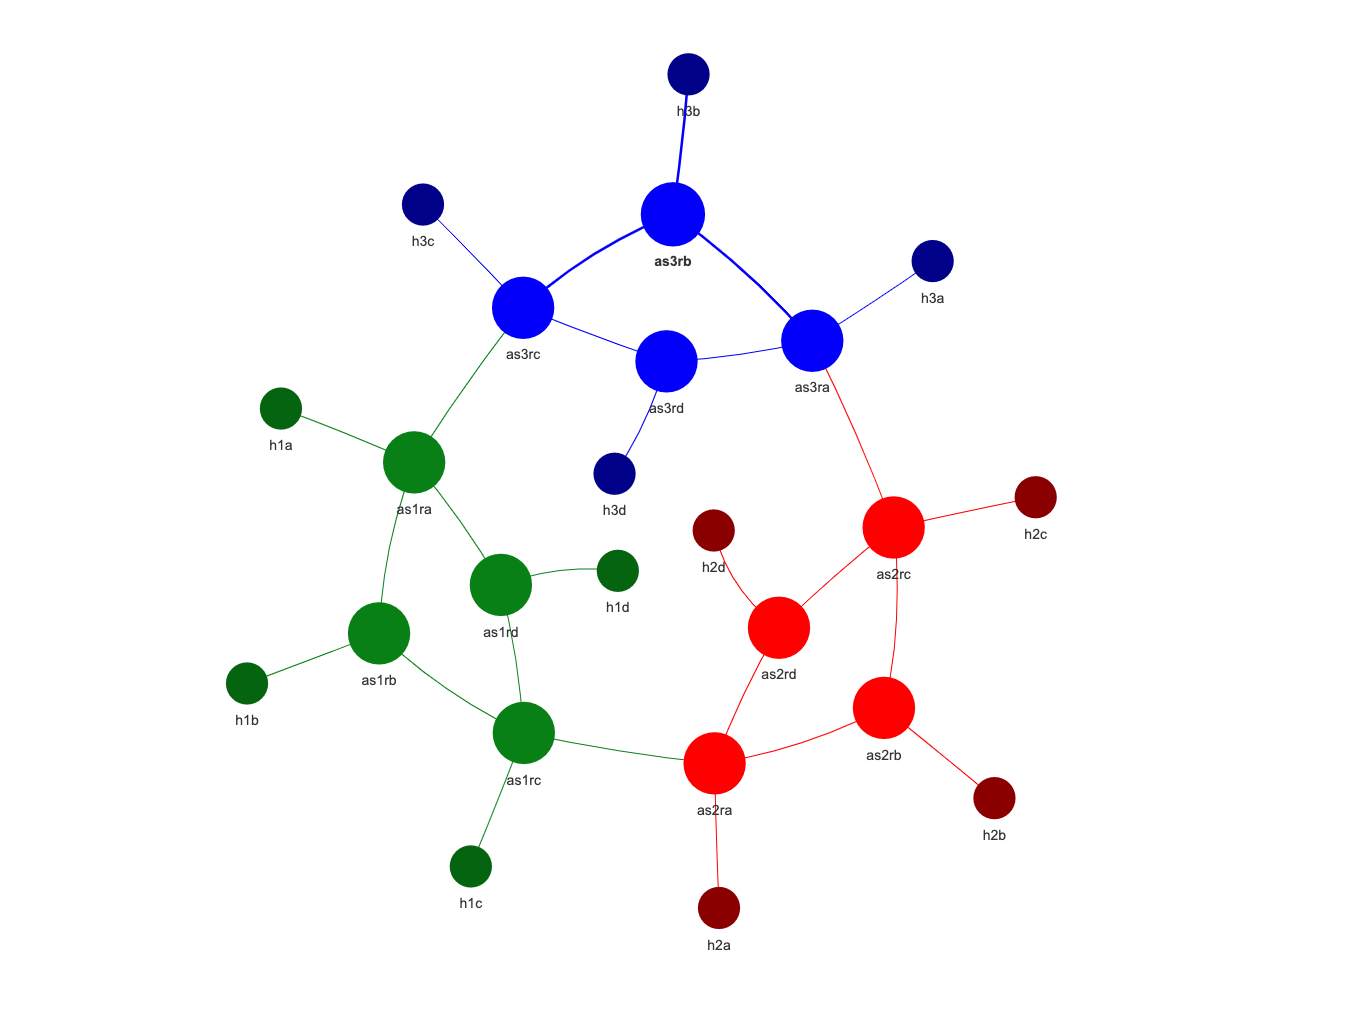
\includegraphics[scale=0.6]{Lab4/graphics/ex5graph.png}
\end{center}

For our scenario, we are checking how the traceroute changes from h1d to h2d. We have set the IGP metric for all intra-AS links to 1 for convenience.

\subsection{Ping from h1d to h2d}

First, we set up a ping from h1d to h2d so that we can monitor for packet loss. Can be found in traces/ping-h1d-h2d.txt.

\subsection{Monitoring OSPF and BGP packets}

Second, we monitor for OSPF packets on as1rd and BGP packets on as1rc using Wireshark. traces/ospf.pcapng and traces/bgp.pcap.

\subsection{Initial Traceroute}

Third, we perform our first traceroute and we obtain the following route:

\begin{verbatim}
    traceroute to fc00:0:2:d::2 (fc00:0:2:d::2), 30 hops max, 80 byte packets
 1  as1rd (fc00:0:1:d::d)  0.056 ms  0.011 ms  0.032 ms
 2  as1rc (fc00:0:1:bc::c)  0.065 ms  0.026 ms  0.014 ms
 3  as2ra (fc00:12::a)  0.042 ms  0.020 ms  0.020 ms
 4  as2rd (fc00:0:2:ad::d)  0.034 ms  0.029 ms  0.024 ms
 5  h2d (fc00:0:2:d::2)  0.035 ms  0.029 ms  0.062 ms
\end{verbatim}


This makes sense, it is indeed the shortest path if we take a look at our first graph.

\subsection{Bringing Down the Inter-AS Link}

Fourth, we go to as2ra and bring down the inter-AS link with as1rc. We notice in our BGP trace that there is an UPDATE message, letting us know that the network is updating the reachability information. When we check the traceroute, we get the following route:

\begin{verbatim}
traceroute to fc00:0:2:d::2 (fc00:0:2:d::2), 30 hops max, 80 byte packets
1  as1rd (fc00:0:1:d::d)  0.057 ms  0.011 ms  0.065 ms
2  as1ra (fc00:0:1:ad::a)  0.075 ms  0.029 ms  0.044 ms
3  as3rc (fc00:13::c)  0.072 ms  0.034 ms  0.031 ms
4  as3rb (fc00:0:3:bc::b)  0.071 ms  0.050 ms  0.024 ms
5  as3ra (fc00:0:3:ab::a)  0.073 ms  0.041 ms  0.034 ms
6  as2rc (fc00:23::c)  0.067 ms  0.228 ms  0.052 ms
7  as2rd (fc00:0:2:cd::d)  0.075 ms  0.048 ms  0.044 ms
8  h2d (fc00:0:2:d::2)  0.166 ms  0.060 ms  0.046 ms
\end{verbatim}


Which makes sense if we look at the following visualization of the network after bringing the link down:

\begin{center}
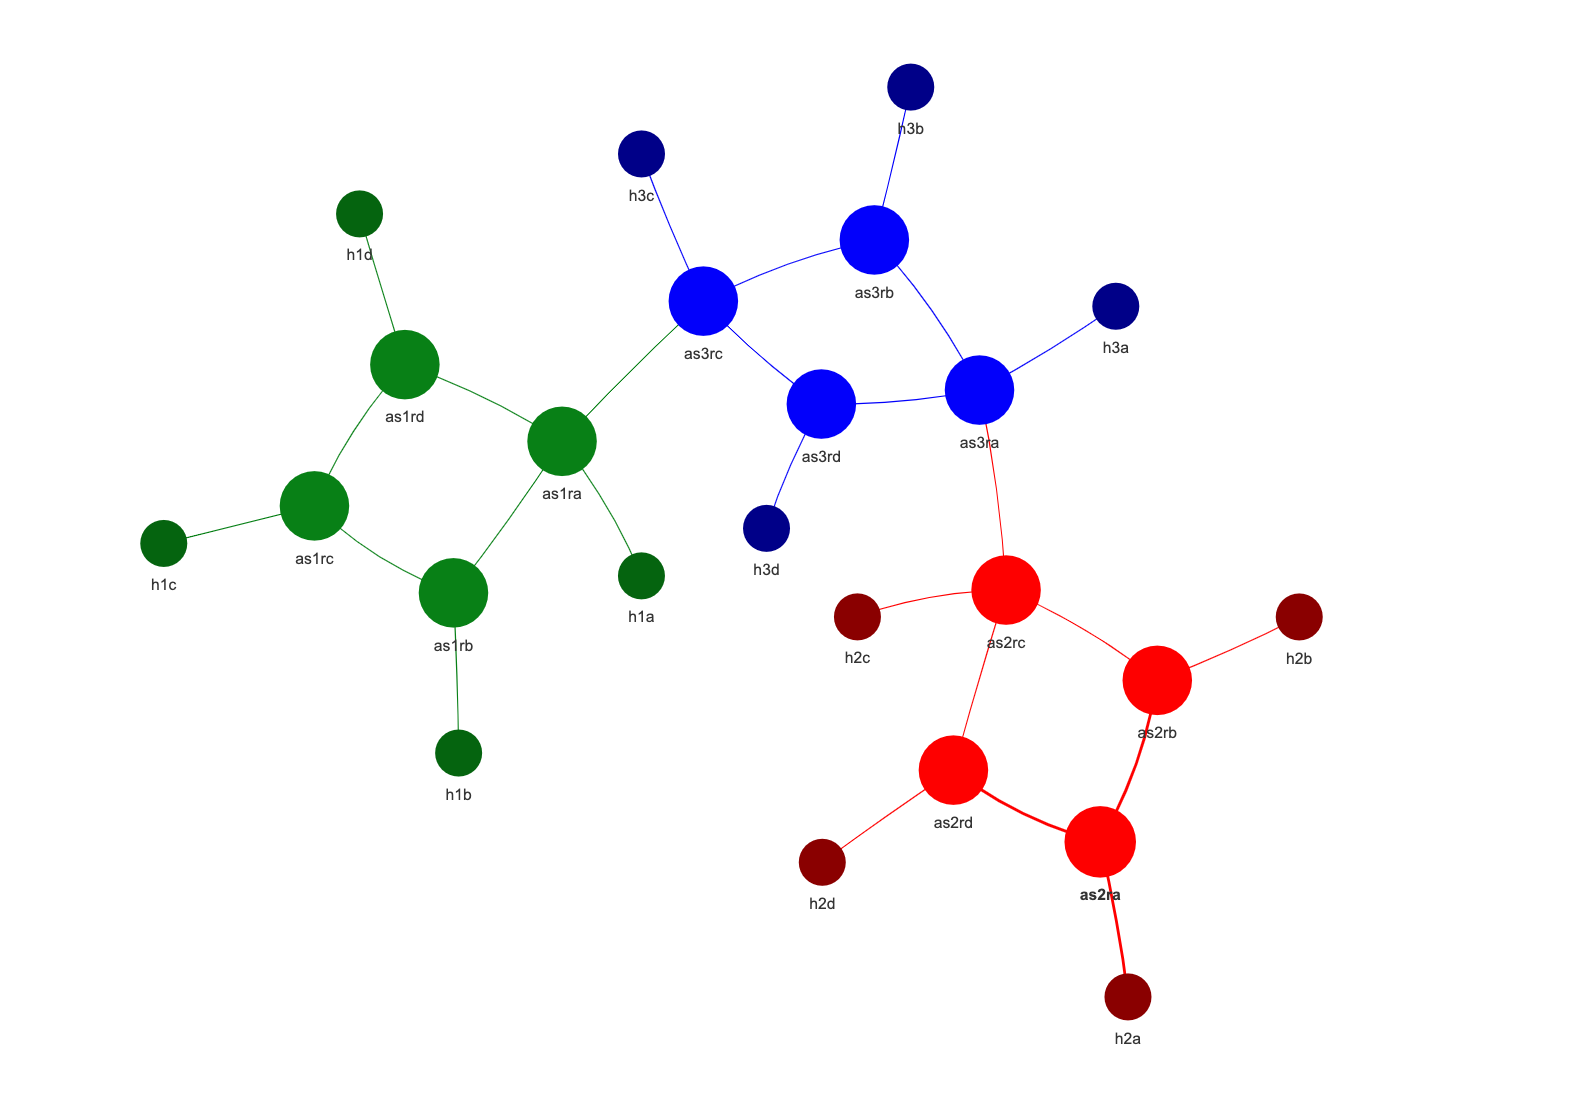
\includegraphics[scale=0.6]{Lab4/graphics/ex5graph2.png}
\end{center}

\subsection{Bringing Down the Intra-AS Link}

Fifth, we go to as1ra and bring down the link with as1rd. This time, this is an intra-AS link, so we quickly see in our OSPF trace that there are LS update packets being sent, which is shortly followed by LS acknowledge packets, letting us know that the new link-state information has been successfully received.

The resulting topology and subsequent traceroute look like this:

\begin{center}
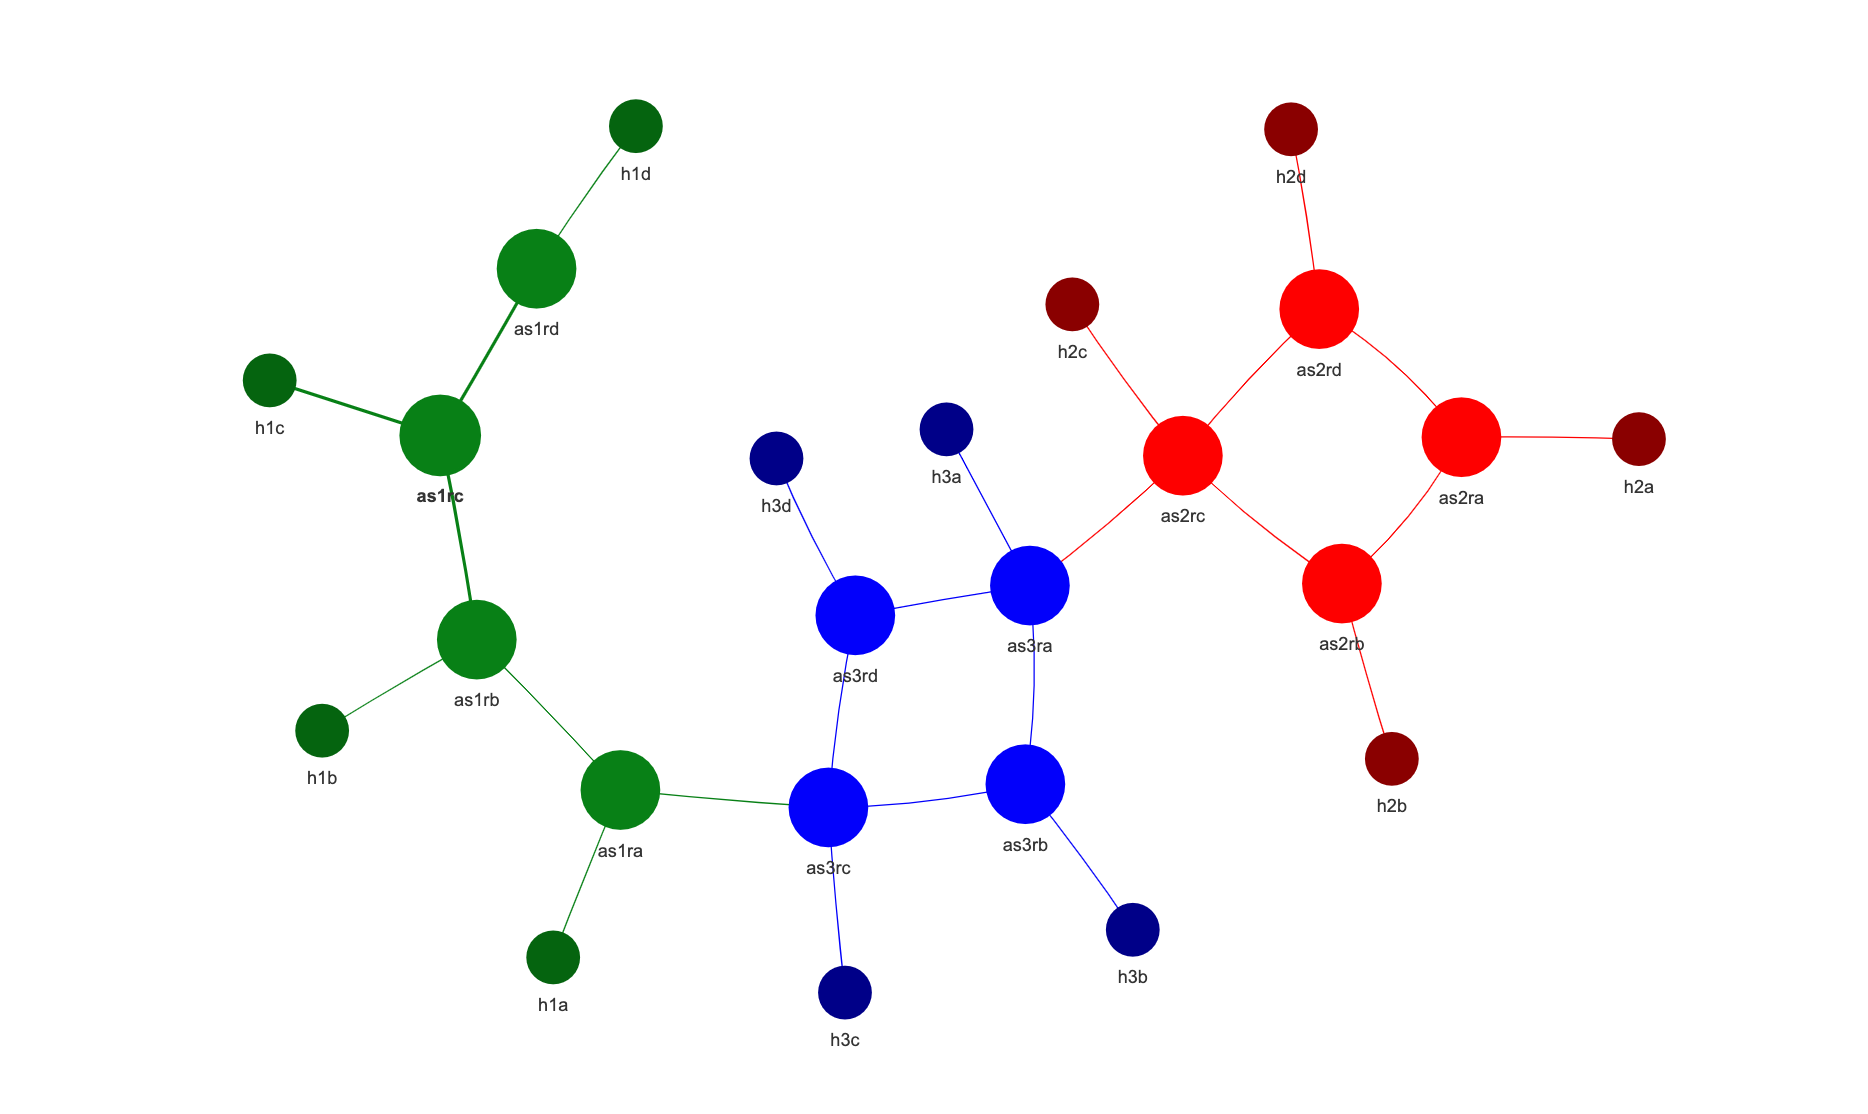
\includegraphics[scale=0.6]{Lab4/graphics/ex5graph3.png}
\end{center}

\begin{verbatim}
traceroute to fc00:0:2:d::2 (fc00:0:2:d::2), 30 hops max, 80 byte packets
1  as1rd (fc00:0:1:d::d)  0.057 ms  0.011 ms  0.065 ms
2  as1rc (fc00:0:1:c::d)  0.074 ms  0.011 ms  0.065 ms
3  as1rb (fc00:0:1:b::d)  0.067 ms  0.011 ms  0.065 ms
4  as1ra (fc00:0:1:ad::a)  0.070 ms  0.029 ms  0.044 ms
5  as3rc (fc00:13::c)  0.072 ms  0.034 ms  0.031 ms
6  as3rb (fc00:0:3:bc::b)  0.071 ms  0.050 ms  0.024 ms
7  as3ra (fc00:0:3:ab::a)  0.073 ms  0.041 ms  0.034 ms
8  as2rc (fc00:23::c)  0.067 ms  0.228 ms  0.052 ms
9  as2rd (fc00:0:2:cd::d)  0.075 ms  0.048 ms  0.044 ms
10  h2d (fc00:0:2:d::2)  0.166 ms  0.060 ms  0.046 ms
\end{verbatim}


\subsection{Restoring Both Links}

Finally, we bring both links back up. This time, it took a couple of minutes for the link states to be updated again since it takes longer to re-establish network adjacencies than it is to notice that you have lost a neighbor. We get the following traceroute, which is the same as the original:

\begin{verbatim}
    traceroute to fc00:0:2:d::2 (fc00:0:2:d::2), 30 hops max, 80 byte packets
 1  as1rd (fc00:0:1:d::d)  0.056 ms  0.011 ms  0.032 ms
 2  as1rc (fc00:0:1:bc::c)  0.065 ms  0.026 ms  0.014 ms
 3  as2ra (fc00:12::a)  0.042 ms  0.020 ms  0.020 ms
 4  as2rd (fc00:0:2:ad::d)  0.034 ms  0.029 ms  0.024 ms
 5  h2d (fc00:0:2:d::2)  0.035 ms  0.029 ms  0.062 ms
\end{verbatim}